\documentclass[12pt,border=4pt,multi]{article}%\documentclass[tikz,border=4pt,multi]{article}
\usepackage{lingmacros}
\usepackage{tree-dvips}
\usepackage{amssymb} %for mathbb{}
\usepackage[dvipsnames]{xcolor}
\usepackage{forest}
\usepackage{amsmath} %for matrices
\usepackage{xeCJK}
\usepackage{tikz}
\usepackage[arrowdel]{physics}
\usepackage{graphicx}
\usepackage{wrapfig}
\usepackage{listings}
\graphicspath{{./img}} %specify the graphics path to be relative to the main .tex file, denoting the main .tex file directory as ./
\usepackage{esint}
\newcommand\Myperm[2][^n]{\prescript{#1\mkern-2.5mu}{}P_{#2}}
\newcommand\Mycomb[2][^n]{\prescript{#1\mkern-0.5mu}{}C_{#2}}
\definecolor{orchid}{rgb}{0.7, 0.4, 1.1}

\begin{document}

\section*{Xi Liu, xl3504, Homework 3}
Problem 1\\
(a)
\begin{lstlisting}[language = c, mathescape = true]
find(int A[], int j, int k, int x)
{
    if(j > k)
        return false;
    int i = j + $\lfloor$ (k - j) / 2 $\rfloor$;
    if(A[i] == x)
        return i;
    if(A[i] < x) 
        return find(A, i + 1, k, x); 
    return find(A, j, i - 1, x);
}
\end{lstlisting}
\leavevmode\\
\\
\\
\\
\\
(b)\\
let $T(n)$ be the running time of the algorithm
\[T(n) = T(n / 2) + 1\]
for a recurrence $T(n) = aT(n / b) + f(n)$, draw an $a$-ary tree, here $a = 1$, so draw a 1-ary tree:\\
\begin{center}
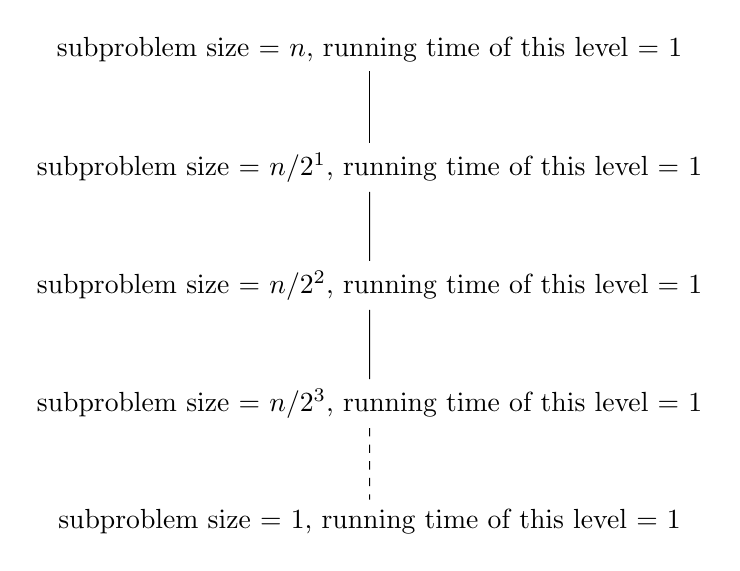
\begin{tikzpicture}
    \node{subproblem size = $n$, running time of this level = 1}
        child{node{subproblem size = $n / 2^1$, running time of this level = 1}
           child{node{subproblem size = $n / 2^2$, running time of this level = 1}
                child{node{subproblem size = $n / 2^3$, running time of this level = 1}
                    child{node{subproblem size = 1, running time of this level = 1} edge from parent [dashed]}
                }
           }
        };
\end{tikzpicture}
\end{center}
\leavevmode
\\
\\
\[n / 2^i = 1, \qquad n = 2^i, \qquad \log_2 n = i\]
\[\text{height} = \log_2 n\]
at depth $i$, cost = (number of nodes)(cost per node) = $(1)(1) = 1$\\
number of leaves = 1\\
\begin{align*}
    T(n) &= \sum_{i = 0}^{\log_2 n - 1} 1 + \Theta(1)\\
    &= (\log_2 n - 1 + 1)(1) + \Theta(1)\\
    &= \log_2 n + \Theta(1)\\
    &= \Theta(\log_2 n)\\
\end{align*}
\[\text{upper bound: } T(n) = O(\log_2 n)\]
\[\text{lower bound: } T(n) = \Omega(\log_2 n)\]
\[T(n) = \Theta(\log_2 n)\]
\newpage
\noindent
(c)\\
the find() algorithm still work if the elements of $A$ are not necessarily distinct, if there are duplicates in the array $A$: $\exists (i,\; j) \in \{[1, A.length] \cap \mathbb{N}\}^2$ such that $A[i] = A[j]$, then the element in $A$ that is equal to $x$ that is first tested by the $if(A[i] == x)$ condition will be selected to return this element's index\\
so the find() algorithm will still outputs the correct return value $i \in \{j...k\}$ such that $A[i] = x$\\ 
\\
\\
\\
\\
\newpage
\noindent
Problem 2\\
(a)\\
since the elements in A are all the same, the partition routine produces one subproblem with $n - 1$ elements and one with 0 elements in each recursive call\\
partitioning costs $\Theta(n)$ time\\
recursive call on an array of size 0 just returns, $T(0) = \Theta(1)$
\begin{align*}
T(n) &= T(n - 1) + T(0) + \Theta(n)\\
&= T(n - 1) + \Theta(n)\\
\end{align*}
\begin{center}
\begin{tikzpicture}
    \node{$n$}
        child{node{$n - 1$}
            child{node{$n - 2$}
                child{node{$n - 3$}
                    child{node{$\vdots$}
                        child{node{1}}
                    }
                }
            }
        }
\end{tikzpicture}
\end{center}
\[\text{height} = n - 1\]
\[\text{at depth $i$, cost = (number of nodes)(cost per node)} = (1)(n - i) = n - i\]
\[\text{number of leaves} = 1\]
\begin{align*}
    T(n) &=\sum_{i = 0}^{n - 1} (n - i)\\
    &= \sum_{i = 0}^{n - 1} n - \sum_{i = 0}^{n - 1} i\\
    &\text{/* since} \sum_{i = 0}^{n} i = \frac{n(n + 1)}{2} \text{ */}\\
    &= n^2 - \frac{(n - 1)((n - 1) + 1)}{2}\\
    &= n^2 - \frac{(n - 1)n}{2}\\
    &= n^2 - \frac{n^2 - n}{2}\\
    &= \frac{2n^2}{2} - \frac{n^2 - n}{2}\\
    &= \frac{2n^2 - n^2 + n}{2}\\
    &= \frac{n^2 + n}{2}\\
    &= \frac{1}{2}n^2 + \frac{1}{2}n\\
    &= \Theta(n^2)\\
\end{align*}
\\
\\
\\
\\
\newpage
\noindent
(b)\\
/* modified version of partition() function */
\begin{lstlisting}[language = c]
#include <stdio.h>
#include <stdlib.h>

void swap(int * A, int i, int j)
{
    int t = A[i];
    A[i] = A[j];
    A[j] = t;
}

typedef struct s
{
    int piv_start;
    int piv_end;
}s; 

s * partition(int * A, int a, int b)
{
    int i = a, k = b, piv = A[b];
    if(b - a <= 1)
    {
        if(A[a] > A[b])
            swap(A, a, b);
    }
    else
    {
        for(int j = a; j <= k; j++)
        {
            if(A[j] < piv)
            {
                swap(A, j, i);
                i++;
            }
            else if(A[j] > piv)
            {
                swap(A, j, k);
                k--;
                j--;
            }
        }
    }
    s * ret = (s *)malloc(sizeof(s));
    ret->piv_start = i;
    ret->piv_end = k;
    return ret; 
}

void quicksort(int * A, int a, int b)
{
    if(a < b)    
    {
        s * st = partition(A, a, b);
        quicksort(A, a, st->piv_start - 1);
        quicksort(A, st->piv_end + 1, b);
        free(st);
    }   
}
\end{lstlisting}
\leavevmode
\\
\\
\\
\\
(c)\\
the running time will be $\Theta(n)$ if we use the modified version of the partition() function obtained in part (b) in the quicksort() algorithm\\
since there is only 1 call to partition() function\\
\\
first call to partition():\\
after 1 iteration of the for loop in partition() function, since every element in the array $A$ is equal to each other, so $A[j] < piv$ will not be true for the entire iteration of the for loop in partition() function, code inside $if(A[j] < piv)$ will not be executed, so $i++$ will not be executed, $i$ is still equal to $a$ at the end of this call of the partition() function\\
similarly, since every element in the array $A$ is equal to each other, so $A[j] > piv$ will not be true for the entire iteration of the for loop in partition() function, code inside $if(A[j] > piv)$ will not be executed, so $k--$ will not be executed, $k$ is still equal to $b$ at the end of this call of the partition() function\\
\\
after this first call to partition() is done, then there is a recursive call to  quicksort($A,\;a$, st-$>$piv\_start - 1), since piv\_start was set to be $i$, and $i$ is equal to $a$ at the end of last partition(), so piv\_start is equal to $a$; so the call is equivalent to quicksort($A,\; a,\; a - 1$), inside this recursive call of quicksort(), $a < b$ is false since $b$ is assigned to be $a - 1$, and $a \not< a - 1$, so this branch of recursion terminates\\
then there is a recursive call to  quicksort($A$, st-$>$piv\_end + 1, $b$) for the other branch, since piv\_end was set to be $k$, and $k$ is equal to $b$ at the end of last partition(), so piv\_end is equal to $b$; so the call is equivalent to quicksort($A,\; b + 1,\; b$), inside this recursive call of quicksort(), $a < b$ is false since $a$ is assigned to be $b + 1$, and $b + 1 \not< b$, so this branch of recursion terminates\\
\\
then no further calls to quicksort()\\
\newpage
\noindent
Problem 3\\
(a)\\
if there exist a number that occurs more than $n/4$ times in $A$, then the same number must occupy more than $n / 4$ cells in the array. imagine if the array is sorted (so that $\forall i \in [1,\;A.length] \cap \mathbb{N}$, $A[i]$ contains the $i$-th smallest element), and use indices $n / 4,\; 2n / 4,\; 3n / 4$ as dividing points that divide the array $A$ of size $n$ into 4 intervals of equal size:\\
$[1,\,n/4],\;[n/4 + 1,\,2n/4],\;[2n/4 + 1,\, 3n/4],\;[3n/4 + 1,\; n]$\\
each interval has size $n / 4$, any number that more than $n / 4$ occurrences has at least $n / 4 + 1$ occurrences, $n / 4 + 1 > n / 4$. so any number that has more than $n / 4$ occurrences cannot fit into 1 interval that can contain at most $n / 4$ elements, so the number with more than $n / 4$ occurrences must cross the boundary created by the indices $n / 4,\; 2n / 4,\; 3n / 4$, so the number with more than $n / 4$ occurrences must be either the $(n/4)$-th, or the $(2n/4)$-th, or the $(3n/4)$-th smallest element(s)\\ 
\\
\\
\\
(b)\\
/* find\_n\_div\_4() is an algorithm that returns true if there exists an element that occurs more than $n/4$ times in $A$ and returns false if there do not exist an element that occurs more than $n/4$ times in $A$ */
\begin{lstlisting}
#include <stdio.h>
#include <stdlib.h>
#include <stdbool.h>
#include <time.h>

void swap(int * ptr, int i, int j)
{
    int t = ptr[i];
    ptr[i] = ptr[j];
    ptr[j] = t;
}

int partition(int * ptr, int a, int b)
{
    int p_i = a; //partition index
    int piv = ptr[b];
    for(int i = a; i <= b - 1; i++)
    {
        if(ptr[i] <= piv)
        {
            swap(ptr, i, p_i);
            p_i++;
        }
    }
    swap(ptr, p_i, b);
    return p_i; 
}

int rand_partition(int * ptr, int a, int b)
{
    int rand_i = 0;
    srand(time(0));
    if(b - a != 0) 
        rand_i = a + rand() % (b - a);
    swap(ptr, rand_i, b);
    return partition(ptr, a, b);
}

int rand_select(int * A, int left, int right, int i)
{
    if(left == right)
        return A[left];
    int rand_i = rand_partition(A, left, right);
    int k = rand_i - left + 1;
    if(i == k)
        return A[rand_i];
    else if(i < k)
        return rand_select(A, left, rand_i - 1, i);
    else
        return rand_select(A, rand_i + 1, right, i - k);
}

bool find_n_div_4(int * A, int n)
{/* n is the length of array pointed by A */
    for(int i = 1; i <= 4; i++) //constant number of iterations
    {
        int num_th = i * (n / 4);
        int sel_num = rand_select(A, 1, n, num_th);
        int count = 0;
        for(int i = 1; i <= n; i++)
        {
            if(A[i] == sel_num)
                count++;
        }
        if(count > n / 4)
            return true;
    }
    return false;
}
\end{lstlisting}
\newpage
\noindent
Problem 4\\
the assumption of $T(k/2) = O(k/2)$ and the last step are wrong, since we have not proved the exact form of the inductive hypothesis, which is $T(k) \leq ck$. we need to explicitly prove
that $T(n) \leq cn$ when we want to show that $T(n) = O(n)$\\
\\
a more explicit use of the substitution method yields the result below:\\
assume $T(k) \leq ck$ for all positive $n < k$, in particular for $n = k / 2$, or equivalently assume $T(k / 2) \leq c(k / 2)$\\
\begin{align*}
T(k) &= 2T(k / 2) + k\\
&\leq 2c(k / 2) + k\\
&= ck + k\\
\end{align*}
$T(k) \leq ck + k$ does not imply $T(k) \leq ck$ for any choice of $c$\\
so the inductive hypothesis is not proved\\
\\
\\
\\
\\
to find a solution to the recurrence\\
\\
$T(n) =
\begin{cases}
1 & \text{if } n = 1\\
2T(n/2) + n & \text{if } n \geq 2\\
\end{cases}$\\
\\
use the substitution method with a different inductive hypothesis\\
guess solution is $T(n) = O(n\lg n)$, need to prove 
\[T(n) \leq cn\lg n\]
base step: when $n = 2$, the proposition is true, since $T(2) = 2T(2/2) + 2 = 2T(1) + 2 = 4 \leq c(2)\lg(2) = 2c; \qquad \forall c \geq 2$ \\
assume $T(m)$ is true for all positive $m < n$, in particular for $m = n / 2$, or equivalently $T(n / 2) \leq c(n / 2)\lg(n / 2)$\\
substitute inductive hypothesis into recurrence
\begin{align*}
   T(n) &= 2\textcolor{orchid}{T(n / 2)} + n\\
   &\leq 2\textcolor{orchid}{c(n / 2)\lg(n / 2)} + n\\
   &\leq cn\lg(n / 2) + n\\
   &= cn(\lg n - \lg 2) + n\\
   &= cn\lg n - cn\lg 2 + n\\
   &= cn\lg n - cn + n\\
   &\leq cn\lg n\\
   &\forall c \geq 2\\
\end{align*}
\newpage
\noindent
Problem 5\\
(a)\\
if $n$ is a power of 2, then $n$ is even, $n = 2^k$\\
{\large
$2^{2^k} = 2^{(2^{k - 1})/2} = \left(2^{(2^{k - 1})}\right)^2$\\ 
}
if $n$ is even, {\large$2^n = (2^2)^{n/2}$}\\
\\
\\
\\
(b)\\
for example, $k = 1$, then $n = 2^k + 2^{k - 1} = 2^1 + 2^0 = 2 + 1 = 3$, which is an odd number, so $n$ can be an odd number in this case\\
if $n$ is odd, {\large$2^n = 2(2)^{n - 1} = 2(2^2)^{(n - 1)/2}$}\\
\\
\\
\\
(c)\\
\begin{lstlisting}[language = c, mathescape = true]
/* mul() computes $a^n$ using $\Theta(\lg n)$ multiplications
the problem need to compute $2^n$, 
so call mul() with $a = 2$ 
which is mul($2, n$)
`%' is the modulo operation that
returns the remainder of a division */

int mul(int a, int n)
{
    if(n < 0)
        return mul(1 / a, -n);
    else if(n == 0)
        return 1;
    else if(n % 2 == 0)     /* even */
        return mul(a * a, n / 2);
    else if(n % 2 == 1)     /* odd */
        return a * mul(a * a, (n - 1) / 2);
}
\end{lstlisting}
\leavevmode
\\
\\
\\
the algorithm mul() have a time complexity of $T(n) = \Theta(\lg n)$ since each recursive call to mul() takes a subproblem size of either $n / 2$ or $(n - 1) / 2$, the tree with the maximum depth divides the problem size by 2 each time (the tree with the maximum depth make the recursive call with subproblem size of $n / 2$)\\
\begin{center}
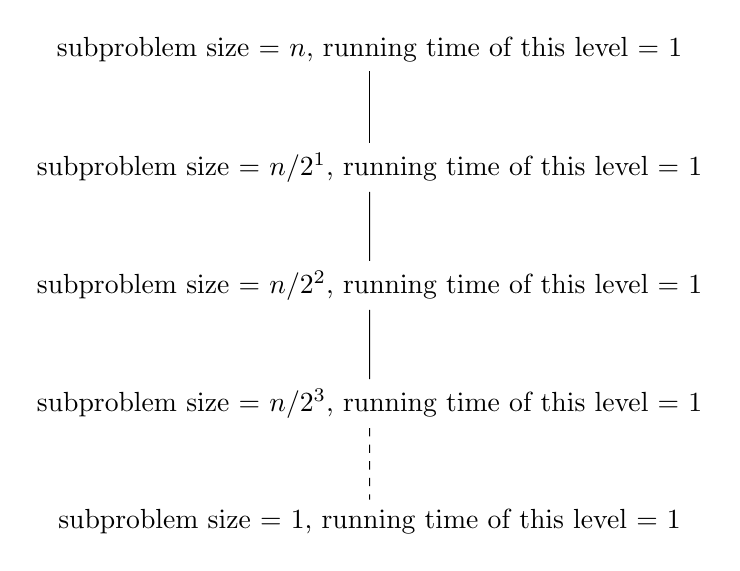
\begin{tikzpicture}
    \node{subproblem size = $n$, running time of this level = 1}
        child{node{subproblem size = $n / 2^1$, running time of this level = 1}
           child{node{subproblem size = $n / 2^2$, running time of this level = 1}
                child{node{subproblem size = $n / 2^3$, running time of this level = 1}
                    child{node{subproblem size = 1, running time of this level = 1} edge from parent [dashed]}
                }
           }
        };
\end{tikzpicture}
\end{center}
\[n / 2^i = 1, \qquad n = 2^i, \qquad \log_2 n = i\]
\[\text{height} = \log_2 n\]
at depth $i$, cost = (number of nodes)(cost per node) = $(1)(1) = 1$\\
number of leaves = 1\\
\begin{align*}
    T(n) &= \sum_{i = 0}^{\log_2 n - 1} 1 + \Theta(1)\\
    &= (\log_2 n - 1 + 1)(1)\\
    &= \log_2 n\\
    &= \Theta(\log_2 n)\\
\end{align*}
\end{document}